%  Remote Sensing (MDPI) manuscript. Compile with the MDPI template folder (Definitions/mdpi.cls) alongside this file.
%  If you do not have the MDPI class, compile remotesensing_manuscript_article.tex instead.
\documentclass[remotesensing, article, submit, moreauthors, pdftex]{Definitions/mdpi}

\firstpage{1}
\makeatletter
\setcounter{page}{\@firstpage}
\makeatother

\pubvolume{18}
\issuenum{x}
\articlenumber{xxxx}
\pubyear{2026}
\externaleditor{Academic Editor: Firstname Lastname}
\history{Received: date; Accepted: date; Published: date}

\usepackage{amsmath}
\usepackage{graphicx}
\usepackage{booktabs}
\usepackage{float}
\providecommand{\needs}[1]{{\color{red}[#1]}}% red placeholders; delete before submission

\Title{Cost-Surface-Driven Network Routing Framework for Rural Clusters Using Extended DS-UNet and StrongDINOv2Seg}

\Author{Pendyala Archana $^{1,*}$ \needs{add co-authors, e.g. supervisor}}

\address{%
$^{1}$ \quad Department of Technology (M.Tech), Chaitanya Bharathi Institute of Technology (CBIT), Hyderabad, India; \needs{e-mail}}

\corres{Correspondence: \needs{e-mail}}

\abstract{\textbf{Background:} Planning internal access routes for rural villages is usually manual, and detection studies seldom connect building extraction to route planning. \textbf{Methods:} We present a framework that derives building and facility targets from 0.6~m imagery with an extended DS-UNet and StrongDINOv2Seg, builds an ordinal 10~m cost surface from land cover and slope with hard constraints, and plans a shared network in two stages in which routes may end on roads or on other routes. The case study is Damarakunta village, Siddipet district, Telangana, India. \textbf{Results:} For 163 house targets, independent least-cost routes total 6753~m of unique length, whereas the proposed network needs 5069~m, a reduction of 24.9\%. All 168 targets connect on the road-line network and no hard constraint is violated. Under synthetic omission and addition of targets the saving remains between 24.9\% and 26.6\%. Keeping routes out of detected buildings lengthens the network by about 22\%. Detection agreement with an independent building layer is 72\%, and no field validation exists. \textbf{Conclusions:} Shared-network planning on a cost surface can substantially shorten rural access networks, but the results are planning alternatives and require labelled buildings and field verification.}

\keyword{geospatial analysis; remote sensing; deep learning; network routing; cost surface; DS-UNet; DINOv2; rural connectivity}

\begin{document}

% Shared manuscript body. Text in red \needs{...} marks items only the authors can supply or confirm.
\providecommand{\needs}[1]{{\color{red}[#1]}}

\section*{Highlights}
\textbf{Main findings}
\begin{itemize}
\item A cost-surface-driven, two-stage planner lets houses attach to existing roads or to other planned routes, cutting the unique new-road length for 163 routed houses in Damarakunta from 6753~m to 5069~m (24.9\%) relative to independently routed access.
\item All 163 house targets and five facility targets were routed with no hard-constraint violations; 168 of 168 route ends connect to the TGRAC road lines, and the saving stays between 24.9\% and 26.6\% under synthetic omission and addition of targets.
\end{itemize}
\textbf{Implications}
\begin{itemize}
\item Counting every independent route in full double-counts shared grid edges (3292~m here) and would overstate the saving about threefold; the unique-length baseline is the fair comparison.
\item Keeping routes out of detected buildings costs about 22\% more network length (6190~m versus 5069~m), so the planner can expose the trade-off between length and building avoidance to decision makers.
\end{itemize}

\section{Introduction}
Rural road connectivity underpins access to schools, health care and markets, yet planning internal village access routes usually relies on manual survey and local judgement. Very-high-resolution (VHR) satellite imagery and open terrain and land-cover products now make it possible to derive building targets, terrain constraints and candidate routes for a whole village from remote sensing data alone.

Deep learning has advanced building extraction from VHR imagery through boundary-aware, attention-based and shape-learning networks \cite{li2024review,ding2022asl,li2022attraction,zhou2022bomsc,zhu2023scil}, and road extraction has progressed through connectivity-preserving and occlusion-aware designs \cite{mei2021coanet,hu2023lgnet,li2024roadcorrector,yang2024occlusion}. Joint building--road extraction has also been studied \cite{guo2024bcr}. Models trained on one region degrade on another, which has motivated domain adaptation and generalization work \cite{ma2023domain,liang2024sdg,zhang2022curriculum}, and recent foundation and vision--language models offer stronger transferable features \cite{oquab2024dinov2,xing2026clip2rs,cao2025ov}. On the planning side, multi-objective path planning on terrain cost surfaces and geographically informed network planning have been proposed for off-road and distribution-network settings \cite{zhu2025pathplan,wang2024distribution}. These strands are rarely combined: detection studies stop at the footprint, and planning studies assume the targets are known.

This paper closes that gap with a framework that runs from imagery to a shared access network. Its objectives are to (i) derive building and facility targets with an extended DS-UNet and a StrongDINOv2Seg model; (ii) build an ordinal terrain cost surface with hard constraints; (iii) plan a network in which routes may end on roads or on other routes; and (iv) evaluate it against baselines, ablations and detection-error stress tests in a case study of Damarakunta village, Siddipet district, Telangana, India. All routes are planning alternatives, not surveyed roads, and costs are ordinal planning units, not rupees.

\section{Materials and Methods}
\subsection{Study Area and Data}
Damarakunta lies in Markook mandal, Siddipet district, Telangana, at about 17.71$^\circ$N, 78.75$^\circ$E. The village boundary from the TGRAC administrative layer is a single polygon of 18.466~km$^2$. Table~\ref{tab:data} lists the inputs. The planning grid is 10~m (679 $\times$ 432 cells, EPSG:32644). The boundary clips the grid, and 44.7\% of the TGRAC road length (93,497~m in 43 lines) lies outside the polygon.

\begin{table}[H]
\caption{Input data for the Damarakunta case study.\label{tab:data}}
\begin{tabularx}{\textwidth}{lXX}
\toprule
\textbf{Layer}	& \textbf{Content}	& \textbf{Source}\\
\midrule
Imagery	& 0.6~m, 3 bands, 11,296 $\times$ 7,171 px mosaic	& Esri World Imagery, exported 4 Oct 2026\\
Boundary	& 1 polygon, 18.466~km$^2$	& TGRAC administrative layer\\
Roads	& 43 line features	& TGRAC (currentness unknown)\\
Facilities	& 2 schools, 1 sub-centre, 2 Gram Panchayat HQ points	& TGRAC\\
Land cover	& 10~m classes	& ESA WorldCover v200 \cite{zanaga2022worldcover}\\
Terrain	& Slope from a 30~m DEM, resampled to 10~m	& SRTM-type DEM \cite{farr2007srtm} (\needs{confirm source})\\
Reference buildings	& Google Open Buildings v3 (agreement checks only)	& \cite{sirko2021openbuildings}\\
\bottomrule
\end{tabularx}
\end{table}

\subsection{Framework Overview}
The framework has five stages: detection, terrain modelling, planning, stress-testing and validation (Figure~\ref{fig:arch}). The planner, its inputs and the reference run are hash-pinned (SHA-256), so each run is reproducible.

\begin{figure}[H]
\centering
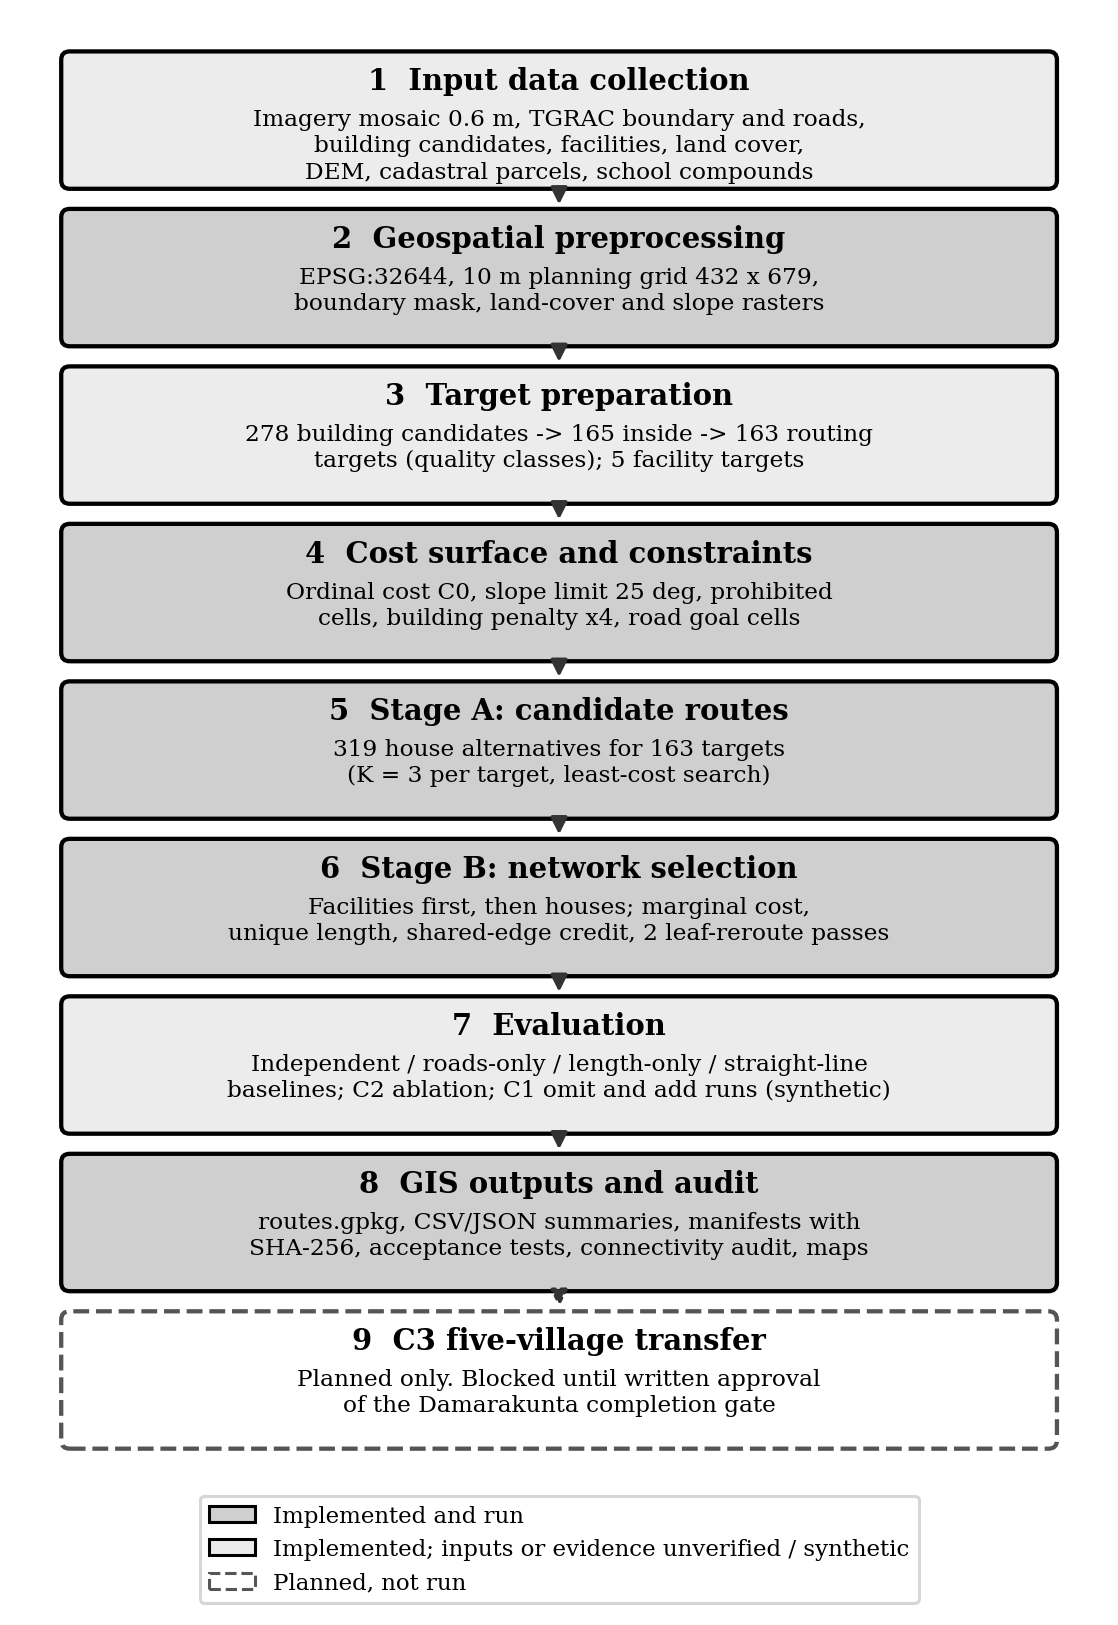
\includegraphics[width=0.55\textwidth]{figures/fig1_architecture.png}
\caption{Framework architecture from input data to GIS outputs. The five-village transfer study (C3) is planned but not run.\label{fig:arch}}
\end{figure}

\subsection{Building and Facility Detection}
\textit{Extended DS-UNet.} \needs{Describe the extended DS-UNet: expansion of ``DS'', the extension made to the U-Net design \cite{ronneberger2015unet}, training data, loss, and implementation details. This repository does not contain the DS-UNet code, so nothing is stated here.}

\textit{StrongDINOv2Seg.} The second model uses a DINOv2-base encoder \cite{oquab2024dinov2} (patch size 14, 768 channels, fine-tuned end to end). Hidden states of transformer layers 3, 6, 9 and 12 are fused by a feature pyramid \cite{lin2017fpn} and an atrous spatial pyramid pooling module \cite{chen2018deeplab}, followed by four residual upsampling blocks and a 1$\times$1 segmentation head with three auxiliary heads. It was trained on LoveDA \cite{wang2021loveda} (8 classes, 560-px input, batch size 2, 10 epochs, AdamW-style learning rate $5\times10^{-5}$, weight decay $10^{-4}$) with a combined loss
\begin{equation}
\mathcal{L} = 0.5\,\mathcal{L}_{\mathrm{CE}} + 0.4\,\mathcal{L}_{\mathrm{Dice}} + 0.1\,\mathcal{L}_{\mathrm{edge}} + 0.4\sum_{k=1}^{3}\mathcal{L}_{\mathrm{aux},k}.
\end{equation}
The best checkpoint reached mIoU 53.80\% and mDice 68.91\% on the LoveDA validation set. These are source-domain scores and are not accuracy in Damarakunta. \needs{confirm the optimizer and the checkpoint metadata; the training log is not in the repository.}

\textit{Targets.} The building extraction produced 278 candidate polygons (165 inside the boundary), grouped by quality into plausible, review and unresolved-merge classes. 163 house targets entered planning. No reference buildings exist for the village, so detection is assessed only by agreement with independent layers.

\subsection{Cost Surface and Constraints}
Each valid 10~m cell $i$ receives an ordinal cost from its land-cover class and slope $s_i$ (degrees):
\begin{equation}
c_i = c_{\mathrm{lc}}(i) + w_s \,\frac{\min(s_i,\,s_{\max})}{s_{\max}}, \qquad w_s = 4,\; s_{\max} = 10^\circ,
\label{eq:cost}
\end{equation}
with base costs $c_{\mathrm{lc}}$ of 8 (tree cover), 6 (cropland), 5 (shrubland), 4 (bare or sparse vegetation), 3 (grassland) and 2 (built-up), giving costs from 2.09 to 12.0. Water, no-data cells and cells steeper than 25$^\circ$ are hard-blocked. Cells touched by a detected footprint receive a penalty multiplier $\lambda$ ($\lambda = 4$ in the primary configuration).

\subsection{Two-Stage Network Planning}
Stage~A generates up to $K=3$ least-cost alternatives per target on the 8-connected grid using a Dijkstra-type search \cite{dijkstra1959}, with the cost of moving between neighbouring cells $i$ and $j$ at distance $d_{ij}$
\begin{equation}
e_{ij} = d_{ij}\,\frac{\lambda_i c_i + \lambda_j c_j}{2},
\label{eq:edge}
\end{equation}
where $\lambda_i=\lambda$ inside penalised cells and 1 elsewhere (\needs{confirm Eq.~\ref{eq:edge} against the planner source}). Stage~B selects routes greedily by weight over marginal cost, with facilities planned first. A route may end on a road or on an already selected route, so shared edges are paid for once. Two leaf-reroute passes then re-attach end segments. The proposed network length is the unique length $L_{\mathrm{net}}$ of all selected edges, compared with the unique length $L_{\mathrm{ind}}^{u}$ of independently routed houses:
\begin{equation}
S = \frac{L_{\mathrm{ind}}^{u} - L_{\mathrm{net}}}{L_{\mathrm{ind}}^{u}} \times 100\%.
\label{eq:saving}
\end{equation}
Baselines are independent least-cost routes, a length-only control, a roads-only shared reference and straight lines.

\subsection{Validation}
Facilities are checked against detected footprints (20~m threshold) and Open Buildings polygons (30~m). Connectivity is tested by the planner, on the raster road component and on the TGRAC road lines, snapping route ends within 15~m. Detection-error sensitivity (C1) omits or adds targets at random (five seeds per setting). The C2 ablation varies $K$ and the number of leaf-reroute passes.

\section{Results}
\subsection{Detection and Facility Agreement}
All five facilities in the final layer lie within 8.5~m of a detected footprint and are corroborated by an Open Buildings polygon. Of the 165 candidates inside the boundary, 118 (71.5\%) agree with an independent polygon; agreement is 71.8\% for plausible, 43.8\% for review and 85.5\% for unresolved-merge candidates (Table~\ref{tab:agree}). Open Buildings lists 1537 polygons inside the boundary, 1186 without a candidate, so the 163 targets must not be read as a house count. An anganwadi was excluded because its TGRAC coordinate lies 371~m from the nearest footprint.

\begin{table}[H]
\caption{Agreement of building candidates with Google Open Buildings v3 (a proxy, not ground truth).\label{tab:agree}}
\begin{tabularx}{\textwidth}{lCCC}
\toprule
\textbf{Group}	& \textbf{Candidates}	& \textbf{Agreeing}	& \textbf{Agreement rate}\\
\midrule
All	& 165	& 118	& 0.715\\
Plausible	& 71	& 51	& 0.718\\
Review	& 32	& 14	& 0.438\\
Unresolved merge	& 62	& 53	& 0.855\\
\bottomrule
\end{tabularx}
\end{table}

\subsection{Baseline versus Proposed Network}
All 163 house targets were routed with no hard-constraint violations. Independent routes total 10,045~m, of which 3292~m duplicates edges used by several houses, leaving 6753~m unique. The proposed network needs 5069~m, so Equation~(\ref{eq:saving}) gives $S = 24.9\%$ (1684~m). The roads-only reference already achieves 22.6\%, so letting houses attach to other routes adds 2.3 percentage points. The length-only control is longer (6980~m) and crosses more footprints than the cost-surface routes (Table~\ref{tab:baselines}, Figure~\ref{fig:lengths}).

\begin{table}[H]
\caption{Network length by method, primary configuration (163 houses, building penalty $\lambda=4$).\label{tab:baselines}}
\begin{tabularx}{\textwidth}{XCCC}
\toprule
\textbf{Method}	& \textbf{Unique length (m)}	& \textbf{Saving (\%)}	& \textbf{Routes crossing footprints}\\
\midrule
Independent least-cost	& 6753.1	& 0.0	& 46\\
Length-only control	& 6979.8	& $-$3.4	& 64\\
Roads-only shared reference	& 5229.3	& 22.6	& 29\\
Two-stage plan (proposed)	& 5069.0	& 24.9	& 28\\
\bottomrule
\end{tabularx}
\end{table}

\begin{figure}[H]
\centering
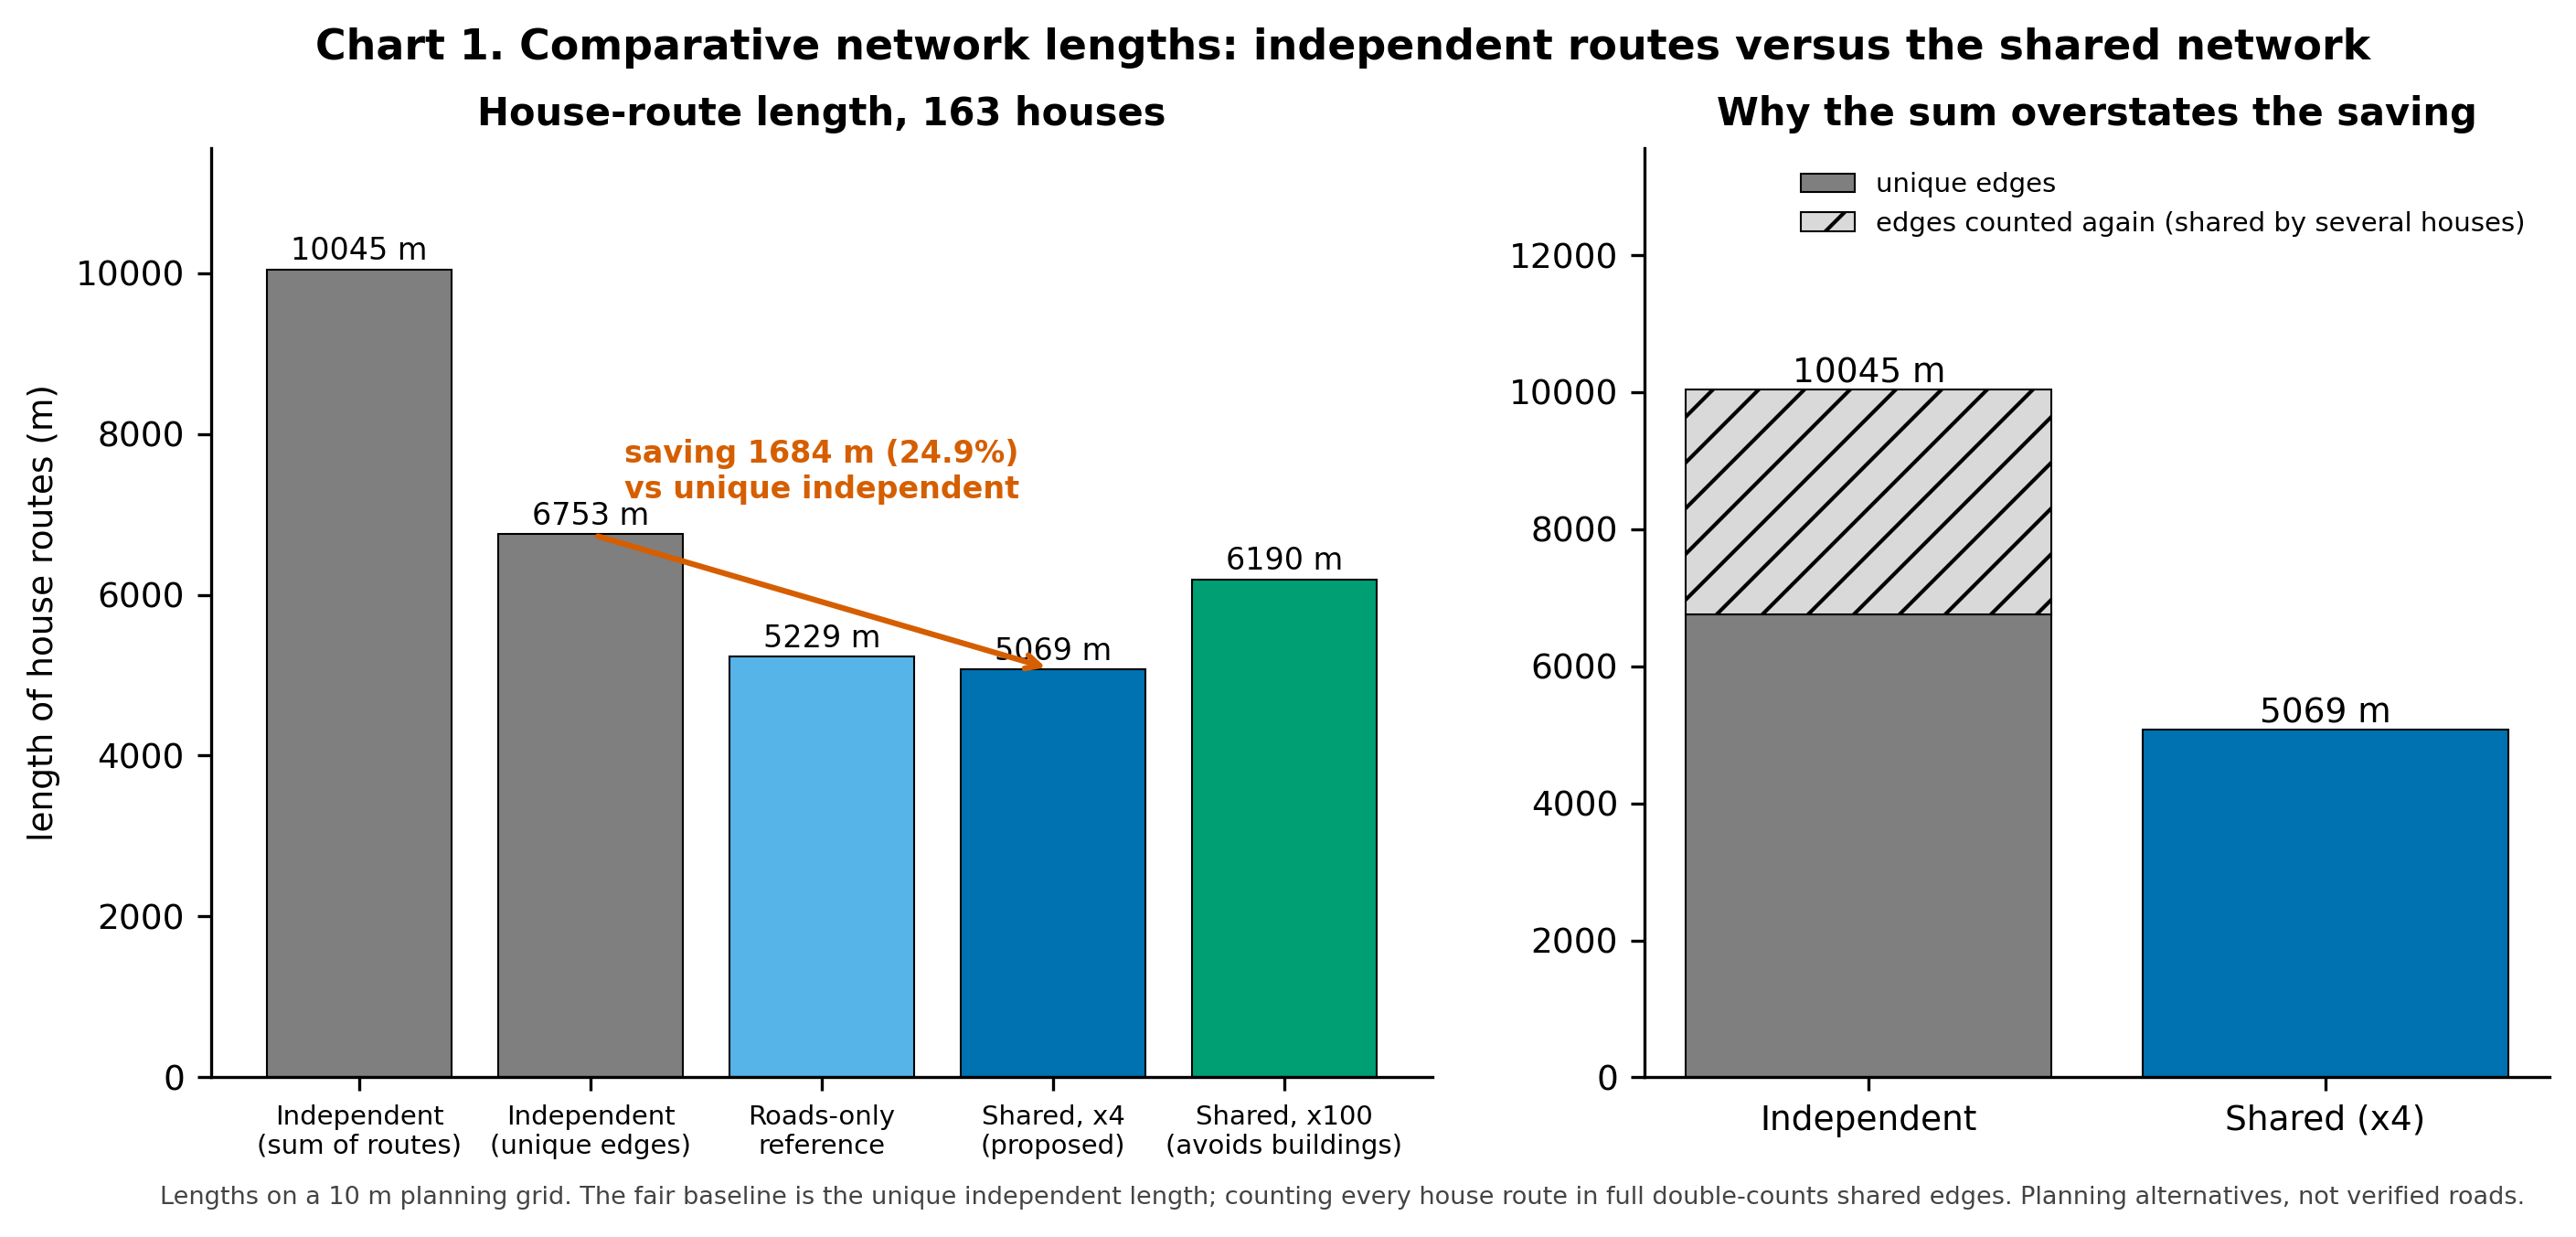
\includegraphics[width=\textwidth]{figures/fig2_network_lengths.png}
\caption{House-route lengths for the independent baselines and shared networks. The sum of independent routes (10,045~m) double-counts shared edges.\label{fig:lengths}}
\end{figure}

\subsection{Connectivity and Constraints}
The planner confirms 168 of 168 targets connected. The raster test finds 167 of 168 on the main road component; the exception is house C0002, whose route ends on a five-cell road fragment cut off by the village polygon. On the TGRAC road lines the fragment belongs to the main network, and 168 of 168 targets connect. No route violates a hard constraint and no cycle exists. The primary plan has 28 house routes crossing other footprints against 56 without the penalty, at 364~m more unique length.

\subsection{Ablation and Obstacle Avoidance}
Two leaf-reroute passes change the length by about 10~m (0.2\%), and $K=3$ instead of $K=1$ changes nothing in this village. Buffering footprints by 7.1~m with $\lambda=100$ gives a 6190~m network (18.9\% saving) with 19 crossing routes instead of 28 (Figure~\ref{fig:avoid}). Raising $\lambda$ above 20 changes nothing, and 16 of the 19 remaining crossings occur within the first 20~m of a route, where a target lies among touching footprints.

\begin{figure}[H]
\centering
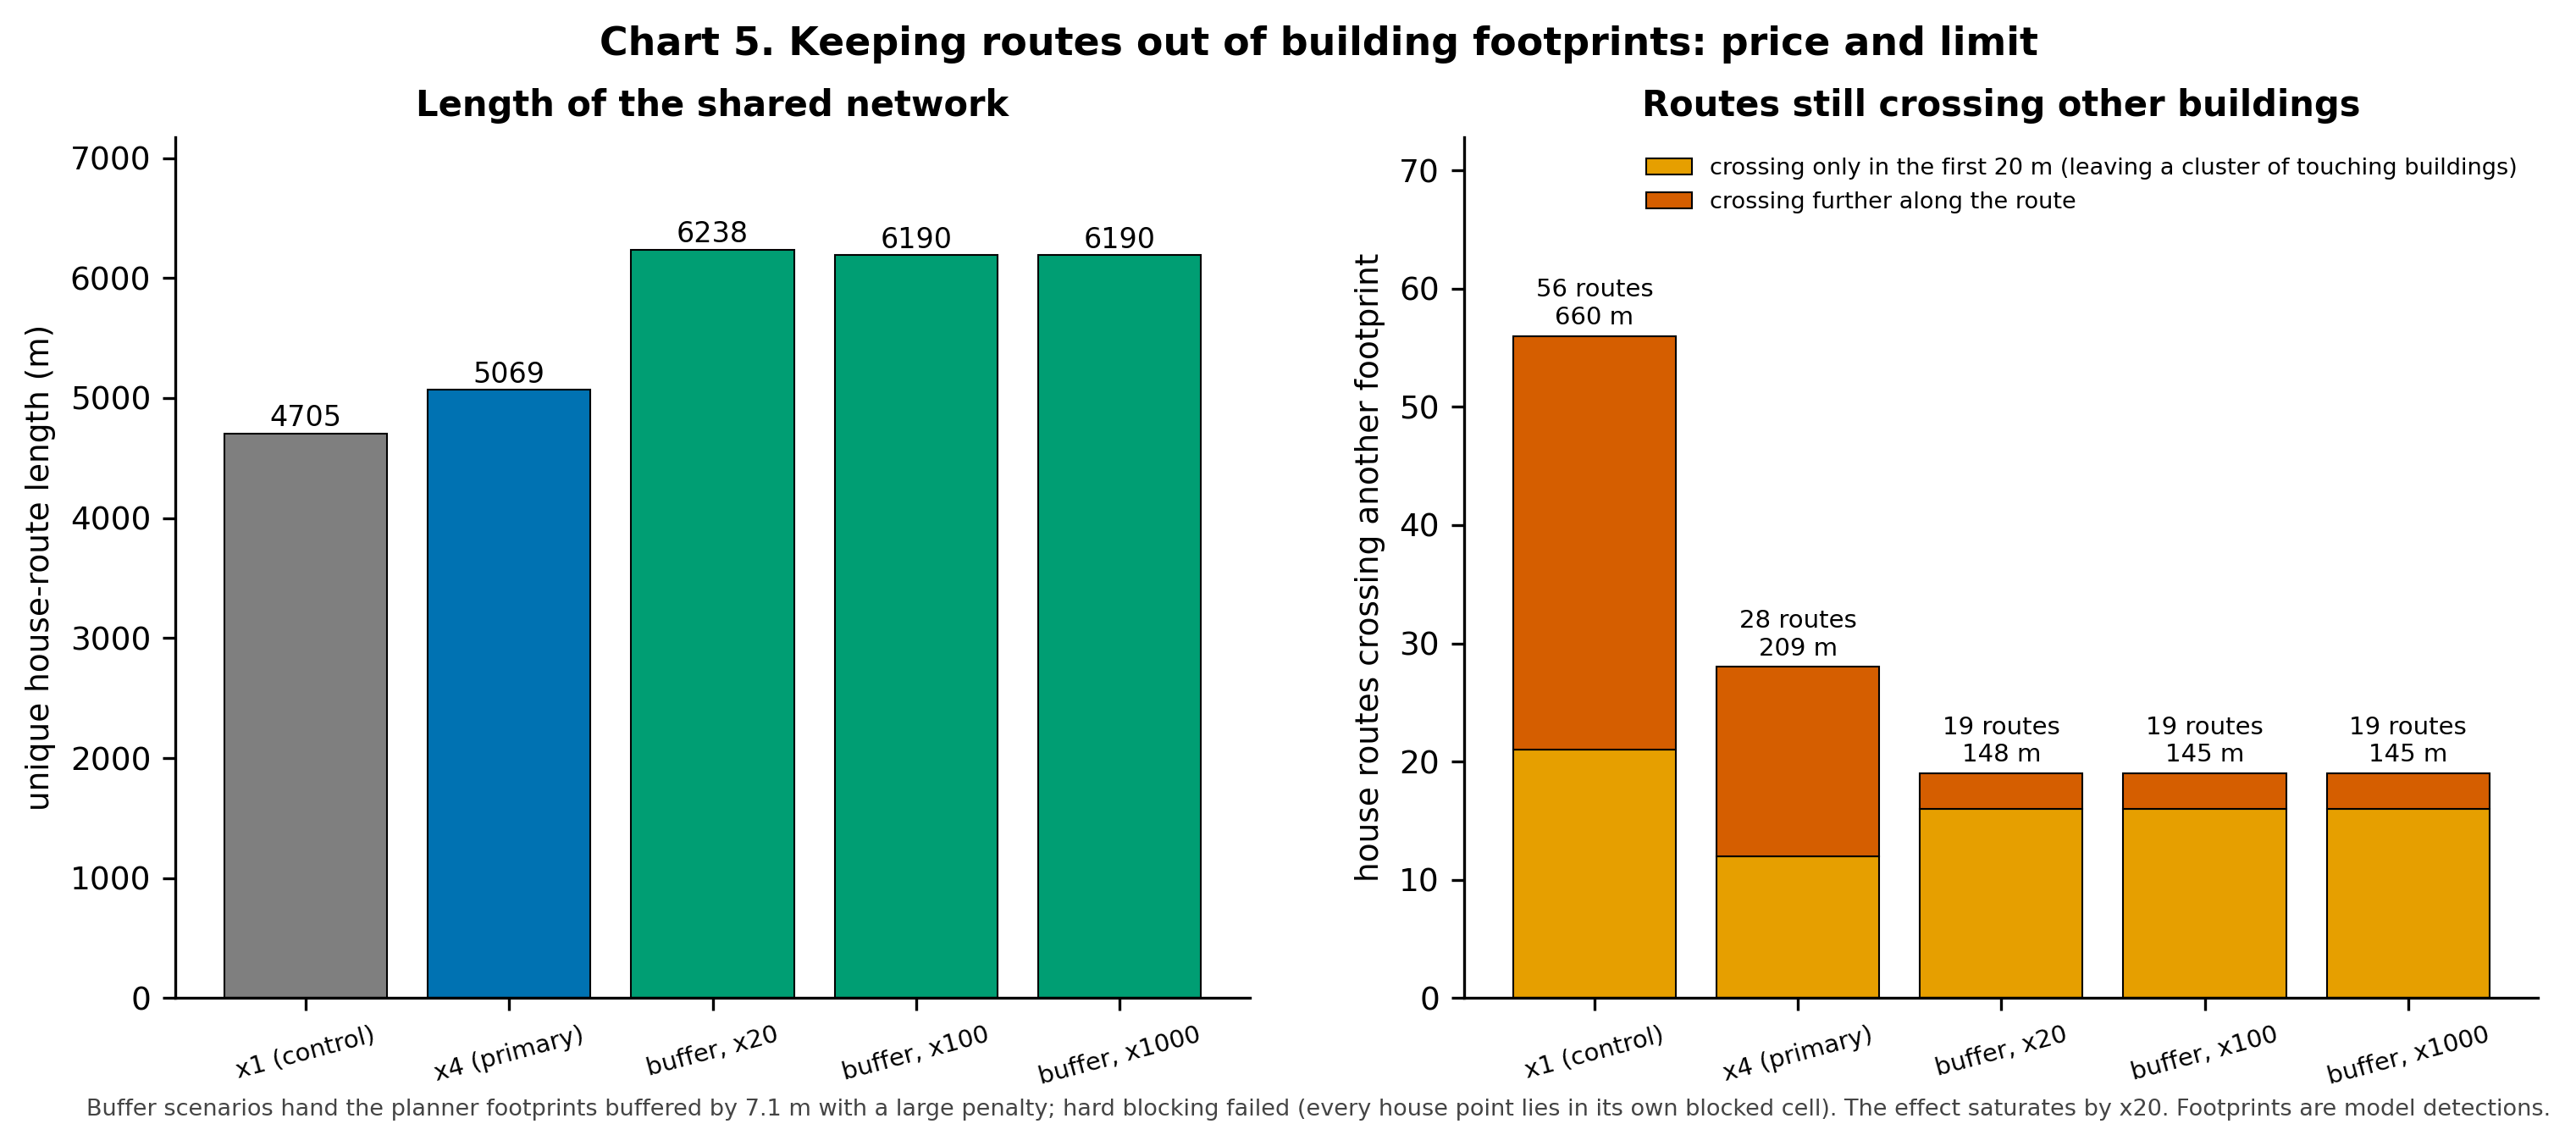
\includegraphics[width=\textwidth]{figures/fig3_avoidance_tradeoff.png}
\caption{Trade-off between network length and building crossings for the penalty scenarios.\label{fig:avoid}}
\end{figure}

\subsection{Sensitivity to Detection Errors}
Every placed target was routed in every perturbation (Table~\ref{tab:c1}). Unique length per routed target stays between 30.8 and 35.4~m (31.1~m at baseline) and the saving between 24.9\% and 26.6\%. The perturbations are synthetic, not measured detector errors.

\begin{table}[H]
\caption{Synthetic omission and addition of targets (C1); means over seeds where more than one run exists.\label{tab:c1}}
\begin{tabularx}{\textwidth}{XCCCC}
\toprule
\textbf{Perturbation}	& \textbf{Targets routed}	& \textbf{Unique length (m)}	& \textbf{Length per target (m)}	& \textbf{Saving (\%)}\\
\midrule
Baseline	& 163.0	& 5069.0	& 31.1	& 24.9\\
Omit 10\%	& 147.0	& 4684.4	& 31.9	& 25.1\\
Omit 20\%	& 130.0	& 4211.5	& 32.4	& 25.0\\
Add 10\%	& 177.4	& 5502.4	& 31.0	& 25.6\\
Add 20\%	& 190.6	& 5868.3	& 30.8	& 25.4\\
Omit merged blobs	& 101.0	& 3579.0	& 35.4	& 26.6\\
\bottomrule
\end{tabularx}
\end{table}

\section{Discussion}
The saving comes from route ends joining roads or other routes, not from overlapping edges: no grid edge is shared by two routes (0.05~m), and 69 of 168 routes end on another route. Most of the gain is already available from the roads-only reference, and the greedy planner is not globally optimal. The unique-length baseline matters: subtracting the shared network from the double-counted total would give 4976~m, three times the real saving of 1684~m.

Detection quality is the main uncertainty. With no reference buildings, 72\% agreement with Open Buildings supports the candidates only partly, and the large number of unmatched Open Buildings polygons shows that targets are missing. The C1 results show the planner degrades gracefully, but a missed house is a missing service that the model cannot detect. The LoveDA scores of StrongDINOv2Seg are source-domain results and should not be read as village-level accuracy.

Other limits apply. The terrain comes from a 30~m DEM resampled to 10~m, costs are ordinal, and imagery licence, capture dates and road currentness are unresolved. No field visit, legal access, drainage or road width has been established, and only one village has been studied. A parametric estimate under assumed unit rates (Rs~75~lakh/km, \needs{confirm source}) puts the length saving at roughly Rs~1.26~crore; it is illustrative and not an engineering estimate.

\section{Conclusions}
A cost-surface-driven framework combining deep-learning detection with two-stage shared-network planning reduced the unique new-road length for 163 houses in Damarakunta by 24.9\% (1684~m) against independent routing, connected all 168 targets on the TGRAC road lines, and kept its saving between 24.9\% and 26.6\% under synthetic detection errors. Avoiding detected buildings raises length by about 22\%. The results are planning alternatives for one village; field validation, labelled buildings and the planned five-village transfer study are needed before wider claims.


\vspace{6pt}
\authorcontributions{Conceptualization, P.A.; methodology, P.A.; software, P.A.; validation, P.A.; formal analysis, P.A.; writing---original draft preparation, P.A.; writing---review and editing, P.A. \needs{adjust to the actual contributions and add co-authors}. All authors have read and agreed to the published version of the manuscript.}

\funding{\needs{State the funding source, or: This research received no external funding.}}

\dataavailability{The input layers and outputs are described in the project repository (Telangana-Rural-Project). The satellite imagery licence is unresolved, so the imagery and maps that contain it cannot be redistributed. TGRAC layers, ESA WorldCover and Google Open Buildings are available from their providers. \needs{Add repository DOI or URL.}}

\conflictsofinterest{The authors declare no conflicts of interest.}

\reftitle{References}
% Shared reference list (MDPI numbered style). Cite with \cite{key}; ranges such as [2-3] are produced by the MDPI class.
\begin{thebibliography}{99}
\bibitem{li2024review} Li, Q.; Mou, L.; Hua, Y.; Shi, Y.; Zhu, X.X. A Review of Building Extraction From Remote Sensing Imagery: Geometrical Structures and Semantic Attributes. \textit{IEEE Trans. Geosci. Remote Sens.} \textbf{2024}, \textit{62}, 1--15. https://doi.org/10.1109/TGRS.2024.3369723.
\bibitem{ding2022asl} Ding, L.; Tang, H.; Liu, Y.; Shi, Y.; Zhu, X.X.; Bruzzone, L. Adversarial Shape Learning for Building Extraction in VHR Remote Sensing Images. \textit{IEEE Trans. Image Process.} \textbf{2022}, \textit{31}, 678--690. https://doi.org/10.1109/TIP.2021.3134455.
\bibitem{li2022attraction} Li, Q.; Mou, L.; Hua, Y.; Shi, Y.; Zhu, X.X. Building Footprint Generation Through Convolutional Neural Networks With Attraction Field Representation. \textit{IEEE Trans. Geosci. Remote Sens.} \textbf{2022}, \textit{60}, 1--17. https://doi.org/10.1109/TGRS.2021.3109844.
\bibitem{zhou2022bomsc} Zhou, Y.; Chen, Z.; Wang, B.; Li, S.; Liu, H.; Xu, D.; Ma, C. BOMSC-Net: Boundary Optimization and Multi-Scale Context Awareness Based Building Extraction From High-Resolution Remote Sensing Imagery. \textit{IEEE Trans. Geosci. Remote Sens.} \textbf{2022}, \textit{60}, 1--17. https://doi.org/10.1109/TGRS.2022.3152575.
\bibitem{zhu2023scil} Zhu, X.; Zhang, X.; Zhang, T.; Tang, X.; Chen, P.; Zhou, H.; Jiao, L. Semantics and Contour Based Interactive Learning Network for Building Footprint Extraction. \textit{IEEE Trans. Geosci. Remote Sens.} \textbf{2023}, \textit{61}, 1--13. https://doi.org/10.1109/TGRS.2023.3317080.
\bibitem{guo2024bcr} Guo, H.; et al. Building-Road Collaborative Extraction From Remote Sensing Images via Cross-Task and Cross-Scale Interaction. \textit{IEEE Trans. Geosci. Remote Sens.} \textbf{2024}, \textit{62}, 1--16. https://doi.org/10.1109/TGRS.2024.3383057.
\bibitem{mei2021coanet} Mei, J.; et al. CoANet: Connectivity Attention Network for Road Extraction From Satellite Imagery. \textit{IEEE Trans. Image Process.} \textbf{2021}, \textit{30}, 8540--8552. https://doi.org/10.1109/TIP.2021.3117076.
\bibitem{hu2023lgnet} Hu, J.; Gao, J.; Yuan, Y.; Chanussot, J.; Wang, Q. LGNet: Location-Guided Network for Road Extraction From Satellite Images. \textit{IEEE Trans. Geosci. Remote Sens.} \textbf{2023}, \textit{61}, 1--12. https://doi.org/10.1109/TGRS.2023.3305031.
\bibitem{li2024roadcorrector} Li, J.; et al. RoadCorrector: A Structure-Aware Road Extraction Method for Road Connectivity Preserving and Updating. \textit{IEEE Trans. Geosci. Remote Sens.} \textbf{2024}, \textit{62}, 1--18. https://doi.org/10.1109/TGRS.2024.3380914.
\bibitem{yang2024occlusion} Yang, R.; et al. Occlusion-Aware Road Extraction Network for High-Resolution Remote Sensing Imagery. \textit{IEEE Trans. Geosci. Remote Sens.} \textbf{2024}, \textit{62}, 1--16. https://doi.org/10.1109/TGRS.2024.3387945.
\bibitem{ma2023domain} Ma, A.; Zheng, C.; Wang, J.; Zhong, Y. Domain Adaptive Land-Cover Classification via Local Consistency and Global Diversity. \textit{IEEE Trans. Geosci. Remote Sens.} \textbf{2023}, \textit{61}, 1--17. https://doi.org/10.1109/TGRS.2023.3265186.
\bibitem{liang2024sdg} Liang, C.; et al. Single Domain Generalization Method for Remote Sensing Image Segmentation. \textit{IEEE Trans. Geosci. Remote Sens.} \textbf{2024}, \textit{62}, 1--16. https://doi.org/10.1109/TGRS.2024.3379669.
\bibitem{zhang2022curriculum} Zhang, B.; et al. Curriculum-Style Local-to-Global Adaptation for Cross-Domain Remote Sensing Image Segmentation. \textit{IEEE Trans. Geosci. Remote Sens.} \textbf{2022}, \textit{60}, 1--12. https://doi.org/10.1109/TGRS.2021.3117851.
\bibitem{xing2026clip2rs} Xing, Y.; et al. CLIP2RS: Leveraging Pretrained Vision-Language Model for Semantic Segmentation of Remote Sensing Images. \textit{IEEE Trans. Geosci. Remote Sens.} \textbf{2026}, \textit{64}, 1--16. https://doi.org/10.1109/TGRS.2025.3647015.
\bibitem{cao2025ov} Cao, Q.; et al. Open-Vocabulary High-Resolution Remote Sensing Image Semantic Segmentation. \textit{IEEE Trans. Geosci. Remote Sens.} \textbf{2025}, \textit{63}, 1--14. https://doi.org/10.1109/TGRS.2025.3559557.
\bibitem{zhu2025pathplan} Zhu, L.; et al. A Multi-Objective Path Planning Framework in Off-Road Environments. \textit{IEEE Trans. Intell. Transp. Syst.} \textbf{2025}, \textit{26}, 19163--19181. https://doi.org/10.1109/TITS.2025.3589586.
\bibitem{wang2024distribution} Wang, Z.; et al. A Practical Urban Distribution Network Planning Method With Geographic Information. \textit{IEEE Trans. Power Syst.} \textbf{2024}, \textit{39}, 7038--7049. https://doi.org/10.1109/TPWRS.2024.3384534.
\bibitem{oquab2024dinov2} Oquab, M.; et al. DINOv2: Learning Robust Visual Features without Supervision. \textit{Trans. Mach. Learn. Res.} \textbf{2024}. arXiv:2304.07193.
\bibitem{wang2021loveda} Wang, J.; Zheng, Z.; Ma, A.; Lu, X.; Zhong, Y. LoveDA: A Remote Sensing Land-Cover Dataset for Domain Adaptive Semantic Segmentation. In Proceedings of the NeurIPS Datasets and Benchmarks Track, 2021. arXiv:2110.08733.
\bibitem{ronneberger2015unet} Ronneberger, O.; Fischer, P.; Brox, T. U-Net: Convolutional Networks for Biomedical Image Segmentation. In \textit{Proceedings of MICCAI 2015}; LNCS 9351; Springer: Cham, Switzerland, 2015; pp. 234--241.
\bibitem{lin2017fpn} Lin, T.-Y.; Doll\'ar, P.; Girshick, R.; He, K.; Hariharan, B.; Belongie, S. Feature Pyramid Networks for Object Detection. In \textit{Proceedings of CVPR 2017}; IEEE: Honolulu, HI, USA, 2017; pp. 2117--2125.
\bibitem{chen2018deeplab} Chen, L.-C.; Papandreou, G.; Kokkinos, I.; Murphy, K.; Yuille, A.L. DeepLab: Semantic Image Segmentation with Deep Convolutional Nets, Atrous Convolution, and Fully Connected CRFs. \textit{IEEE Trans. Pattern Anal. Mach. Intell.} \textbf{2018}, \textit{40}, 834--848.
\bibitem{dijkstra1959} Dijkstra, E.W. A Note on Two Problems in Connexion with Graphs. \textit{Numer. Math.} \textbf{1959}, \textit{1}, 269--271.
\bibitem{sirko2021openbuildings} Sirko, W.; et al. Continental-Scale Building Detection from High Resolution Satellite Imagery. arXiv 2021, arXiv:2107.12283.
\bibitem{zanaga2022worldcover} Zanaga, D.; et al. ESA WorldCover 10 m 2021 v200. Zenodo 2022. https://doi.org/10.5281/zenodo.7254221.
\bibitem{farr2007srtm} Farr, T.G.; et al. The Shuttle Radar Topography Mission. \textit{Rev. Geophys.} \textbf{2007}, \textit{45}, RG2004.
\end{thebibliography}


\end{document}
